\documentclass{beamer}

\usepackage[utf8]{inputenc}
\usepackage{amsmath}
\usepackage{amsfonts}
\usepackage{amssymb}
\usepackage{graphicx}
\usepackage{ragged2e}  % `\justifying` text
\usepackage{booktabs}  % Tables
\usepackage{tabularx}
\usepackage{tikz}      % Diagrams
\usetikzlibrary{calc, shapes, backgrounds}
\usepackage{amsmath}
\usepackage{amssymb}
\usepackage{dsfont}
\usepackage{url}       % `\url
\usepackage{listings}  % Code listings
\usepackage[T1]{fontenc}
\usepackage{theme/beamerthemehbrs}
\usepackage{varwidth}
% \subtitle{Study Project: Deep Learning for Robot Vision}


\title{Continuous Authentication using Mouse Dynamics}
\author{
Istvan Habram \\
Marvin Haschker\\
Kunal Runwal \\
Shalaka Satheesh \\
Samuel Wiest \\
}

\institute[HBRS]{Hochschule Bonn-Rhein-Sieg}

\date{28.06.2022}
% \subject{Test beamer}

% leave the value of this argument empty if the advisors
% should not be included on the title slide
\def\advisors{Florian Dehling, Vincent Scharf, Prof.~Dr.-Ing.~Sebastian Houben}

% \thirdpartylogo{path/to/your/image}


\begin{document}
{
\begin{frame}
\titlepage
\end{frame}
}


\section{Introduction}
\begin{frame}{Continuous Authentication}
    % \begin{itemize}
    %     \item[1.] Bot detection: To identify various users based on available mouse movements 
    %     \item[2.] User authentication: To authenticate a given user based on mouse movements 
    % \end{itemize}
    \begin{block}{Aim}
    Verify the authenticity of a user after login without interfering with the user's work (binary classification as legitimate or imposter). 
    \end{block}
    \begin{columns}[onlytextwidth]
    \column{.35\textwidth}
    Methods of continuous authentication
    \begin{itemize}
        \item Keyboard strokes
        \item Mouse dynamics
    \end{itemize}
    \column{.65\textwidth}
    \begin{figure}
        \centering
        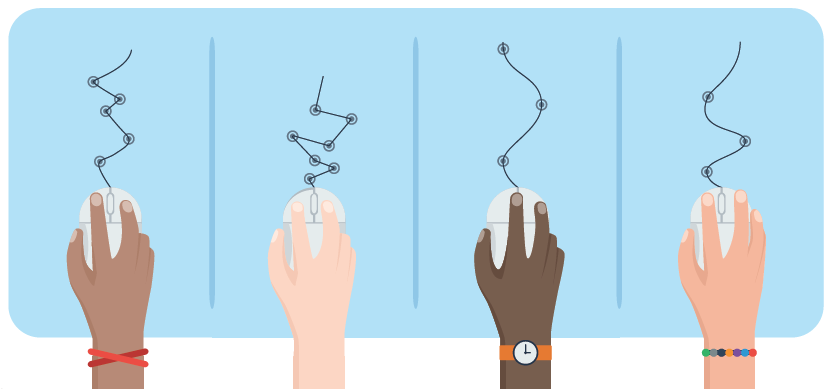
\includegraphics[width=\textwidth]{theme/images/mouse dynamics.png}
        \caption{Mouse dynamics \cite{tommy_riggs}.}
        \label{fig:mouse_dynamics}
    \end{figure}
    \end{columns}
\end{frame}



\section{Dataset}
\begin{frame}{Dataset}
    \begin{itemize}
        \item Number of participants: 153
        \item Session lengths: From 15 seconds to 50 minutes
        \item Some participants have two sessions
    \end{itemize}
    \begin{figure}
        \centering
        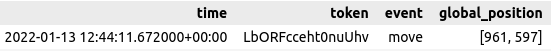
\includegraphics[width=0.8\textwidth]{theme/images/move.png}
        \caption{Move data}
        \label{fig:move}
    \end{figure}
    \begin{figure}
        \centering
        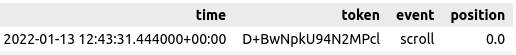
\includegraphics[width=0.8\textwidth]{theme/images/scroll.png}
        \caption{Scroll data}
        \label{fig:scroll}
    \end{figure}
    \begin{figure}
        \centering
        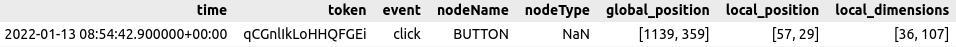
\includegraphics[width=\textwidth]{theme/images/click.png}
        \caption{Click data}
        \label{fig:click}
    \end{figure}
    % \end{columns}
\end{frame}

\begin{frame}{Dataset}
\framesubtitle{Cleaning the data}
    \begin{itemize}
        \item Change data types
        \begin{table}[!ht]
            \centering
            \resizebox{0.3\textwidth}{!}{
            \begin{tabular}{ll}
            \hline
            \textbf{Data}   & \textbf{Data Type} \\ \hline
            Time            & datatime64         \\
            Pixel Positions & int                \\
            Scroll          & float32            \\ \hline
            \end{tabular}}
            \caption{Data and respective data types}
            \label{tab:data-cleaning}
        \end{table}
        \item Remove:
        \begin{itemize}
            \item unneeded columns: `event', `nodeName', `nodeType', `global\_position',`local\_position',
        `local\_dimensions', `Unnamed: 0'
            \item NaN values
        \end{itemize}
        \item Split data into triplets: from global coordinates and time to $(dx, dy, dt)$
        \item Normalize position data
        \item Calculate scroll and move speed $(dx/dt, dy/dt, position/dt)$
    \end{itemize}
\end{frame}


\section{Approach}

\begin{frame}{Approach}
\begin{itemize}
    \item User authentication treated as a binary classification task, identifying the user as \textit{genuine} or \textit{imposter}.
    \item Classical methods use random forests trained directly on the dataset \cite{thomasBroadReviewNonintrusive2021}.
    \item Newer methods propose using a deep neural network for feature extraction, and a one-class SVM for classification \cite{antalSapiMouseMouseDynamicsbased2021}.
    \item Our approach:
    \begin{itemize}
        \item CNN-based feature extractor and one-class SVM classifier.
        \item Random forest trained directly on the dataset.
        \item Random forest trained on the features extracted from the CNN.
    \end{itemize}
\end{itemize}
\end{frame}

\section{Model}

\begin{frame}{Random Forest}
\framesubtitle{Trained on original dataset}
\begin{itemize}
    \item 80/20 train-test split, 64 estimators
    \item Input: move data split into blocks of 128 (dx, dy) pairs
    \item Mean accuracy across batches: 0.992
\end{itemize}

\begin{figure}
    \centering
    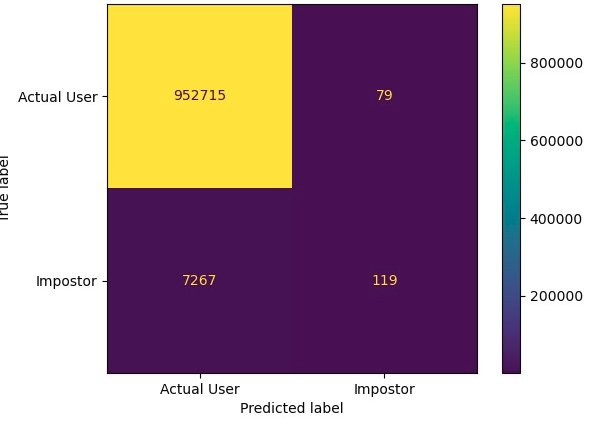
\includegraphics[width = .5\textwidth]{theme/images/confusion_matrix_rfm.png}
    \caption{Confusion matrix}
    \label{fig:confusion_matrix_rfm}
\end{figure}

\end{frame}

\begin{frame}{Random Forest}
\framesubtitle{Trained on extracted features}
\begin{itemize}
    \item 80/20 train-test split, 64 estimators
    \item Input: (128,2) sized move features extracted by the DNN
    \item Mean accuracy across batches: 0.993
\end{itemize}

\begin{figure}
    \centering
    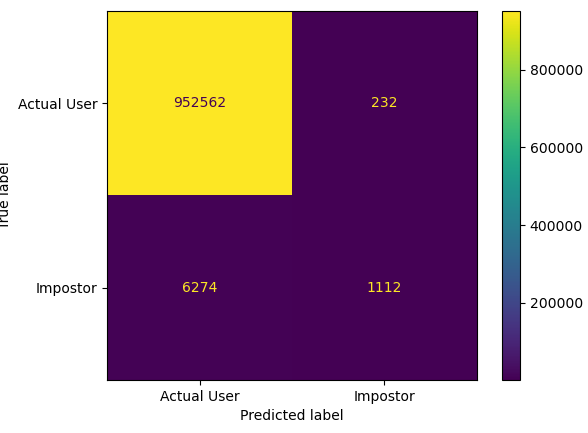
\includegraphics[width = .5\textwidth]{theme/images/confusion_matrix_cnn.png}
    \caption{Confusion matrix}
    \label{fig:confusion_matrix_rf_cnn}
\end{figure}

\end{frame}

\begin{frame}{Deep Neural Network}
\framesubtitle{Convolutional Neural Network}
    \begin{itemize}
        \item Used as a feature extractor
        \item Input shaped (128, 2) for each movement (block size of 128 and dx, dy values)
        \item Output also shaped as (128, 2)
        \item Loss function: categorical cross entropy
    \end{itemize}
    \begin{table}[!ht]
    \centering
    \resizebox{0.5\textwidth}{!}{%
    \begin{tabular}{@{}ll@{}}
    \toprule
    \textbf{Hyperparameter} & \textbf{Value} \\ \midrule
    Size of input & (128, 2) \\
    Learning Rate & 0.0001 (later reduced) \\
    Epochs & 200 \\
    Batch Size & 512 \\
    Optimizer & Adam \\ \bottomrule
    \end{tabular}%
    }
    \caption{Hyperparameters for training feature extractor.}
    \label{tab:feature-extractor}
    \end{table}
\end{frame}

\begin{frame}
\begin{figure}
    \centering
    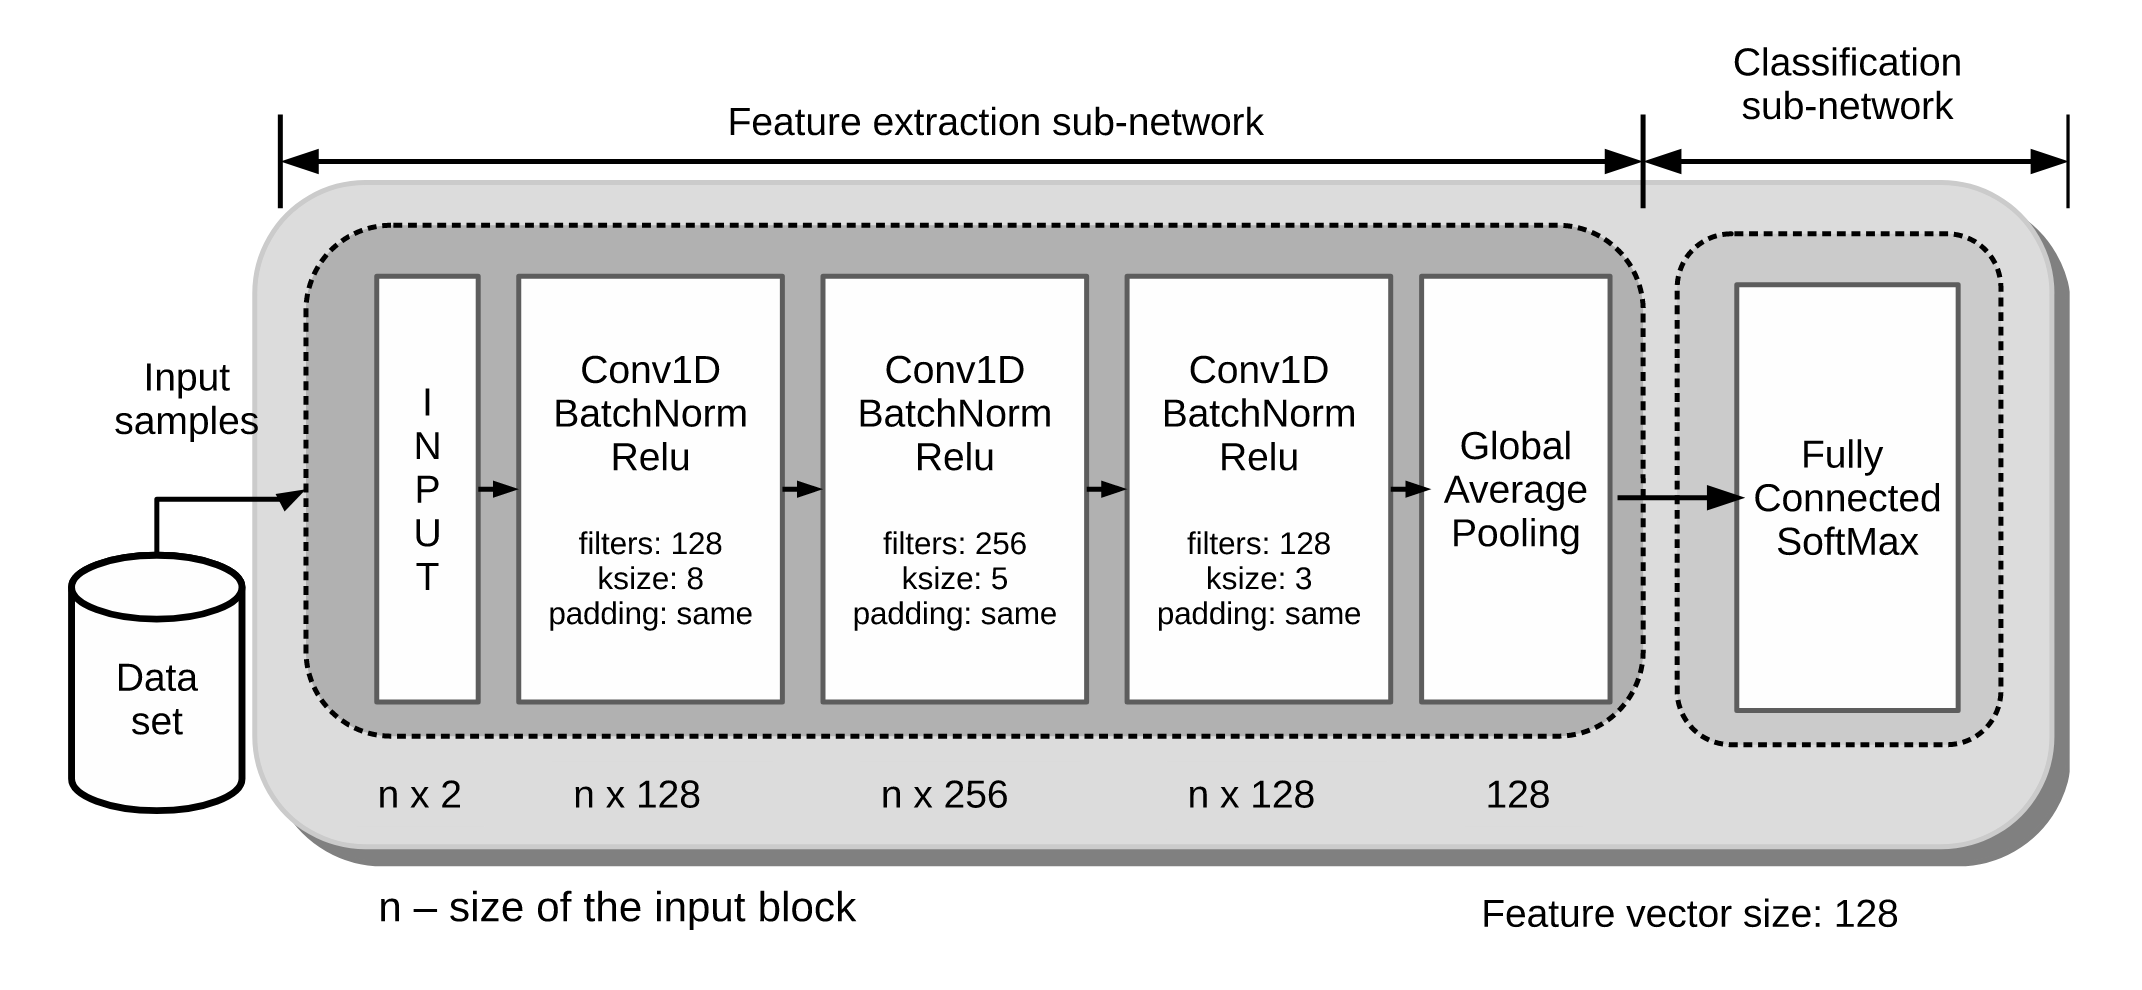
\includegraphics[width=\textwidth]{theme/images/architecture.png}
    \caption{CNN architecture (taken from \cite{antalSapiMouseMouseDynamicsbased2021})}
    \label{fig:architecture}
\end{figure}
\end{frame}

\begin{frame}{Deep Neural Network}
\framesubtitle{Loss during training}
\begin{figure}
    \centering
    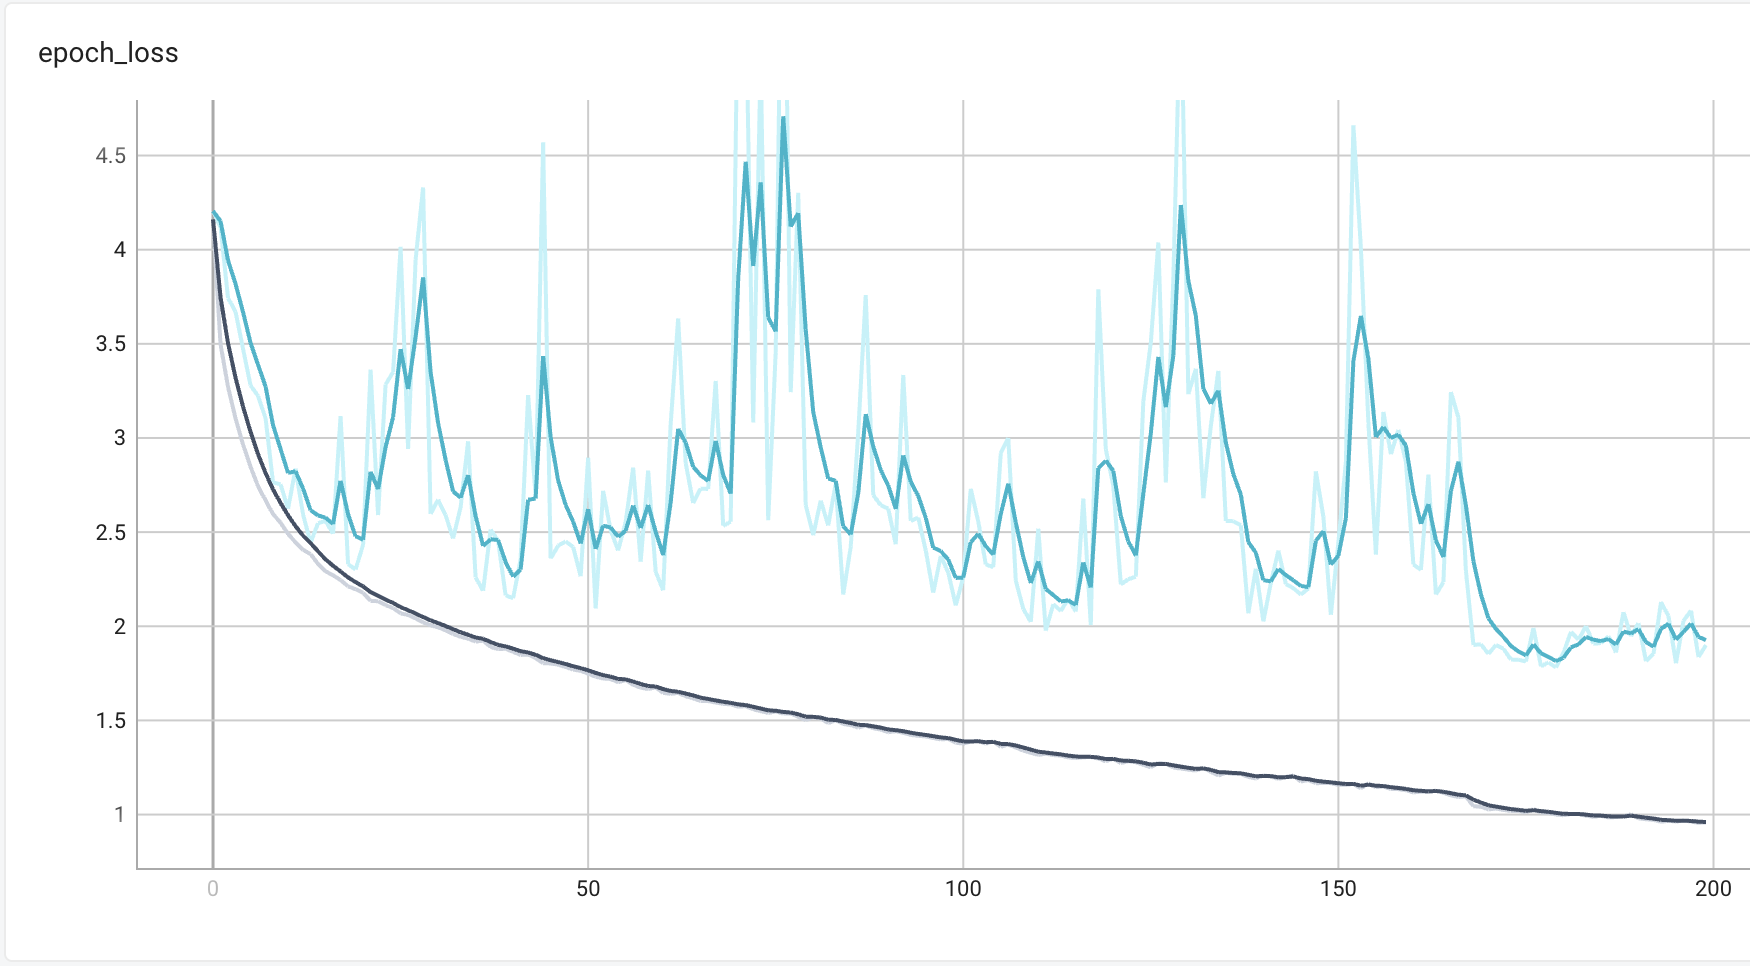
\includegraphics[width=\textwidth]{epoch_loss.png}
    \caption{Epoch loss}
    \label{fig:epoch_loss}
\end{figure}
\end{frame}

\begin{frame}{Deep Neural Network}
\framesubtitle{Accuracy during training}
\begin{figure}
    \centering
    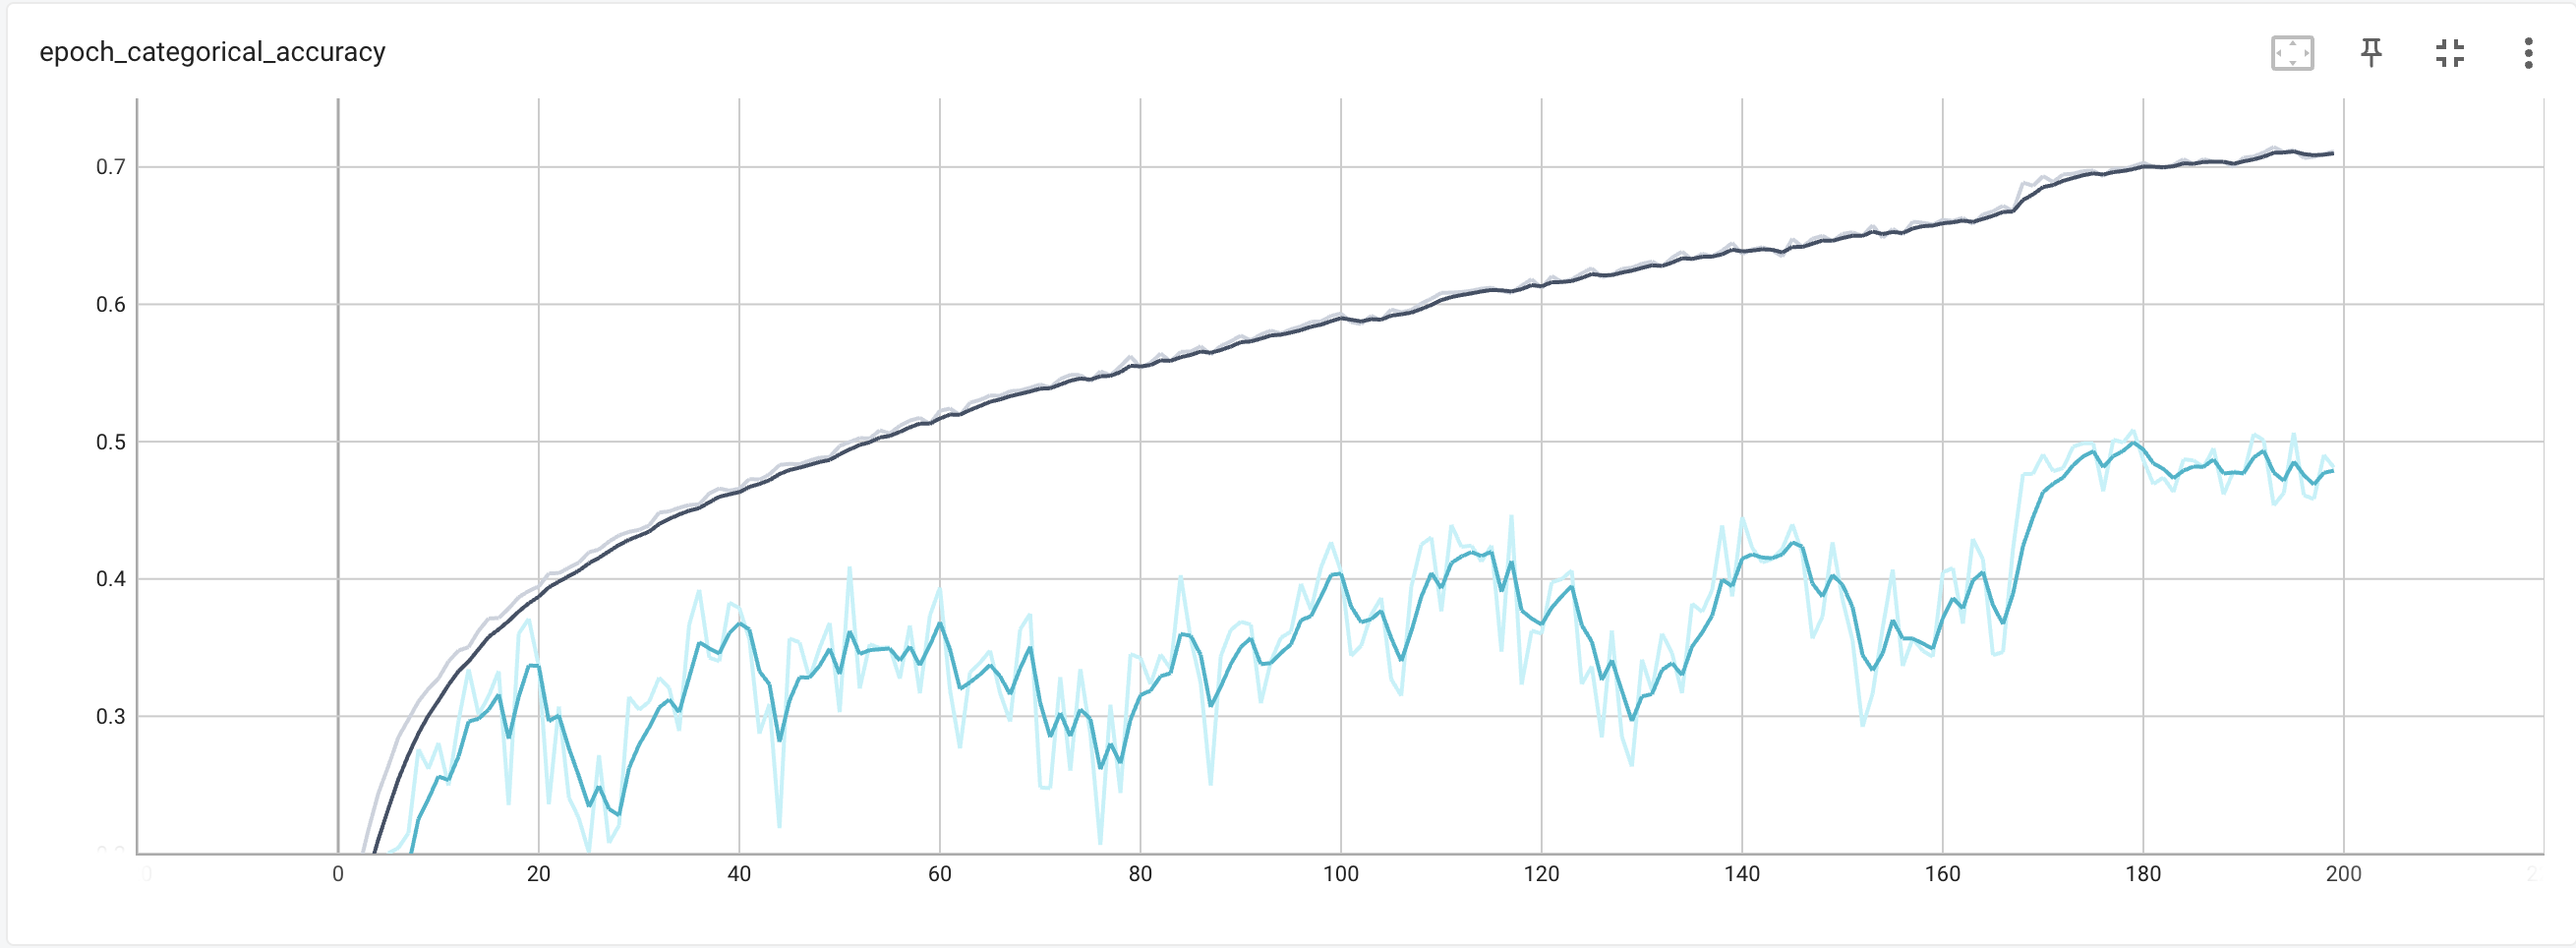
\includegraphics[width=\textwidth]{epoch_categorical_accuracy.png}
    \caption{Epoch categorical accuracy}
    \label{fig:epoch_categorical_accuracy}
\end{figure}
\end{frame}

\begin{frame}{Deep Neural Network}
\framesubtitle{OneClassSVM (based on libsvm)}
    \begin{itemize}
        \item Detection of outliers
        \item Decision boundary computed based on the extracted features
        \item $-1$ for imposter, $1$ for genuine user
        \item Radial basis function kernel
        \item Gamma value of $\frac{1}{2\sigma^2}$ (with $\sigma^2$ being variance of dataset)
    \end{itemize}
\end{frame}

\begin{frame}{Deep Neural Network}
\framesubtitle{Results}
\begin{itemize}
    \item Mean accuracy: $0.95$, AUC: $0.873$
\end{itemize}
\begin{varwidth}{0.5\textwidth}
\begin{figure}
    \centering
    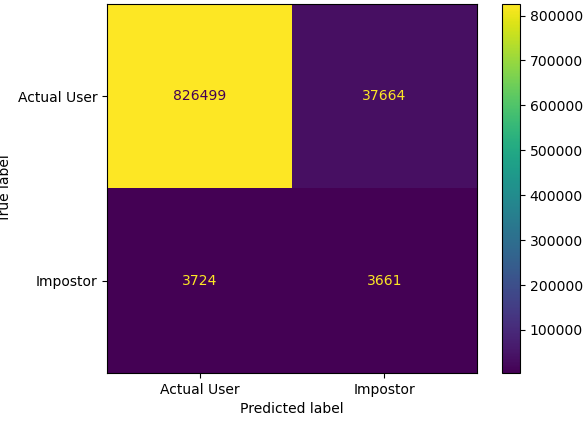
\includegraphics[width=.9\textwidth]{theme/images/cnn_confusion_matrix.png}
    \caption{Confusion matrix of the DNN-SVM.}
    \label{fig:confusion_matrix_svm_cnn}
\end{figure}
\end{varwidth}
\begin{varwidth}{0.5\textwidth}
\begin{figure}
    \centering
    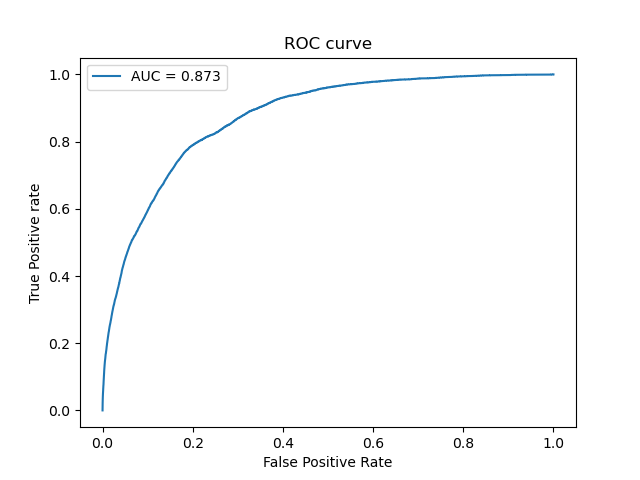
\includegraphics[width=.9\textwidth]{theme/images/roc_curve.png}
    \caption{AUC of the DNN-SVM.}
    \label{fig:dnn_auc}
\end{figure}
\end{varwidth}
\end{frame}

\section{Results}
\begin{frame}{Results}
\begin{itemize}
    \item The DNN-SVM had errors evenly divided between error types, while the RF mainly misclassified a legitimate user as an imposter.
    \item DNN-SVM had a mean accuracy of 0.95 vs a mean accuracy of 0.99 for the random forests.
\end{itemize}
\begin{varwidth}{0.49\textwidth}
\begin{figure}
    \centering
    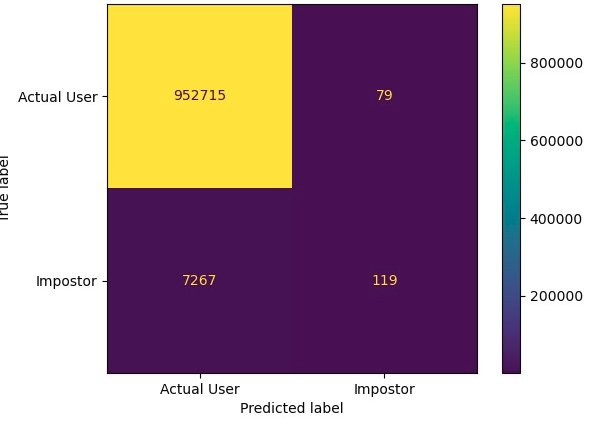
\includegraphics[width = \textwidth]{theme/images/confusion_matrix_rfm.png}
    \caption{RF move dataset}
    \label{fig:confusion_matrix_rfm}
\end{figure}
\end{varwidth}
\begin{varwidth}{0.49\textwidth}
\begin{figure}
    \centering
    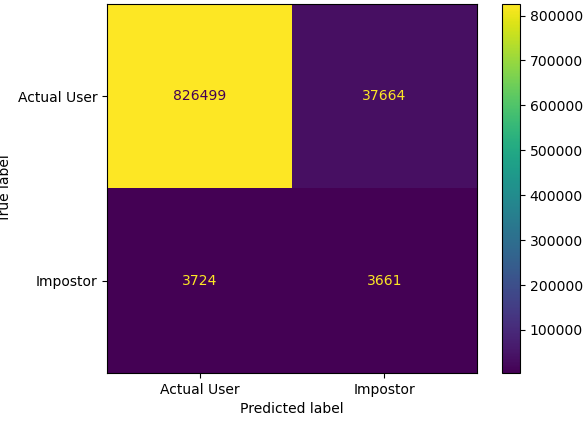
\includegraphics[width=\textwidth]{theme/images/cnn_confusion_matrix.png}
    \caption{DNN-SVM}
    \label{fig:confusion_matrix_svm_cnn}
\end{figure}
\end{varwidth}
\end{frame}


\section{Summary}
\begin{frame}{Conclusion}
    \begin{itemize}
        \item Observations
        \begin{itemize}
            \item DNN features provide a very slight increase in accuracy in the random forest, but this may be a random effect.
            \item The RFs lean towards stricter security at the cost of user convenience. 
        \end{itemize}
        \item Challenges
        \begin{itemize}
            \item Limited user data. DNN results may be improved if more data was available. Other approaches use up to 1000 users with 1 hour recorded for each user \cite{zhengEfficientUserVerification2011}.
        \end{itemize}
        \item Future Work
        \begin{itemize}
            \item Convert the move dataset to velocities instead of positions as mentioned in \cite{antalSapiMouseMouseDynamicsbased2021} and retrain the models.
            \item Implement k-means instead of a one-class SVM for classification with the DNN.
            \item Compare the inference times and the relationship between accuracy and block size for the different approaches.
        \end{itemize}
    \end{itemize}
\end{frame}

\section{Bibliography}

\begin{frame}[allowframebreaks]{Bibliography}
\bibliography{ref.bib}
\bibliographystyle{plain}
\end{frame}

\end{document}
